\documentclass{bsuir}
\usepackage{ulem}
\usepackage{makecell}
\usepackage{multirow}

\departmentlong{инженерной психологии и эргономики}
\worktitle{Практическая работа \textnumero1\\\textquote{Патентное исследование и
патентная информация}}
\titleleft{ Проверила:\\
    Фомин Д.А.\\
    ~
}
\titleright{
    Выполнил:\\
    Бородин А.Н.\\
    гр. 310901
}
\titlepageyear{2025}

\usepackage{pgfplots}
\usepackage{amsmath}
\usepackage{breqn}

\newlength{\tablewidth}
\setlength{\tablewidth}{\textwidth - \parindent}

\begin{document}

\maketitle
\mainmatter

\includepdf[pages=2-,angle=90]{work.pdf}

\chapter*{Заключение}


Проведенные патентные исследования по теме «Упаковщик пультов радиоуправления в
защищённые капсулы для перевозки» выявили следующие ключевые тенденции и
результаты:

В мировой практике активно развиваются технологии автоматизации упаковочных
процессов. Патенты США, Германии и Китая демонстрируют использование независимо
контролируемых механизмов, прецизионной сортировки и адаптивных систем подачи.

Особое внимание уделяется защите хрупких объектов: русский патент описывает
метод упаковки изделий в пластиковые ёмкости с повышенной устойчивостью к
внешним воздействиям.

Выявлен дефицит решений, специфичных для упаковки пультов радиоуправления.
Большинство аналогов ориентировано на общие задачи, что подчеркивает
необходимость разработки специализированного оборудования. Публикации Института
машиноведения им. А.А. Благонравова РАН (2013) подтверждают актуальность
автоматизации линий типа «формование"=фасовка"=укупорка», что соответствует
мировым трендам.

Зарубежный опыт, описанный в работах ВИНИТИ РАН (2008), указывает на растущий
спрос на интеллектуальные системы мониторинга упаковки, включая интеграцию RFID
и IoT.

Предлагаемый в немецком патенте упаковщик обладает потенциалом для в нише защиты
электронных устройств при транспортировке. Его отличительные особенности:

\begin{itemize}
    \item Использование ударопрочных материалов для капсул.
    \item Внедрение системы динамической балансировки для минимизации вибраций.
    \item Адаптируемость алгоритмов сортировки под геометрию пультов радиоуправления.
    \item Проект соответствует глобальным трендам в области «умной упаковки»,
          что повышает его конкурентоспособность.
\end{itemize}

\end{document}
